\begin{frame}
\frametitle{Remy compared with an omniscient protocol}
\begin{itemize}
\item Training/testing scenario:
\begin{tabular}{p{0.3\textwidth}p{0.7\textwidth}}
Link speed & 32 Mbits/sec \\
Minimum RTT & 150 ms \\
Topology & Dumbbell \\
Senders & 2 \\
Workload & 1 sec ON/OFF times \\
Buffer size & 5 BDP \\
Objective & \pbox{0.7\textwidth}{$\sum log(tpt) - log(delay)$ \\ (proportionally fair $\frac{tpt}{delay}$)}
\end{tabular}
\end{itemize}
\end{frame}

\begin{frame}
\frametitle{The omniscient protocol}
\begin{itemize}
\item Protocol knows topology, number, location of senders/receivers  
\item Every time a sender turns ON/OFF,
      \begin{equation*}
      max. \sum log (tpt)
      \end{equation*}
      (Proportionally fair throughput allocations)
\item Set each sender's rate using obtained solution
\item Zero queuing delay
\end{itemize}
\end{frame}

\begin{frame}
\frametitle{Remy approaches omniscient protocol}
\begin{centering}

\noindent \only<1>{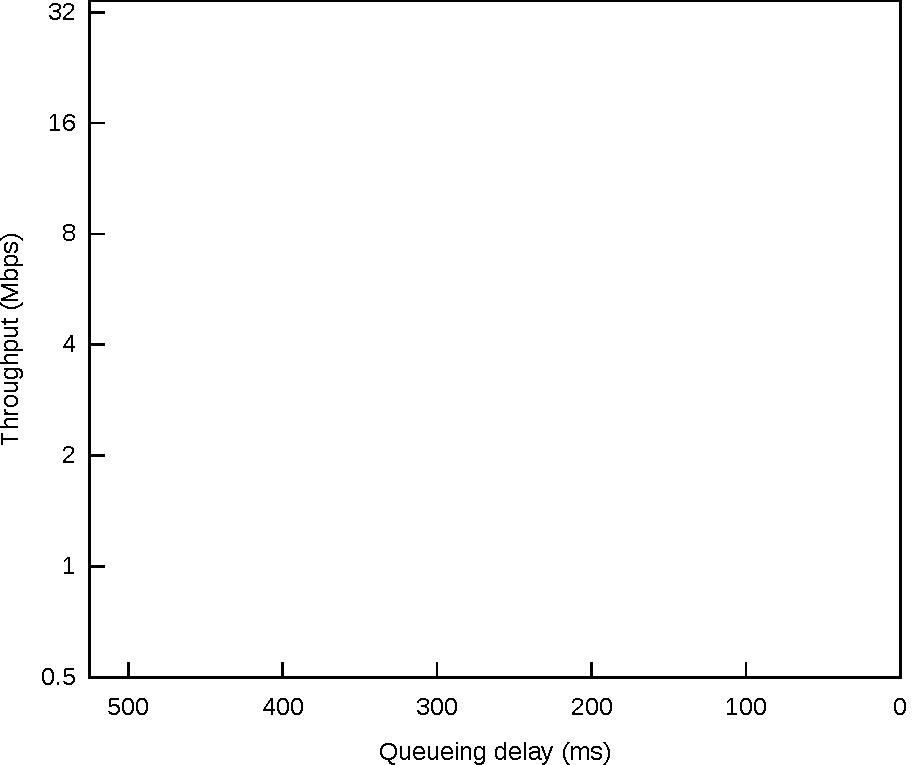
\includegraphics[width=3.3 in]{optimality-base.pdf}}\only<2>{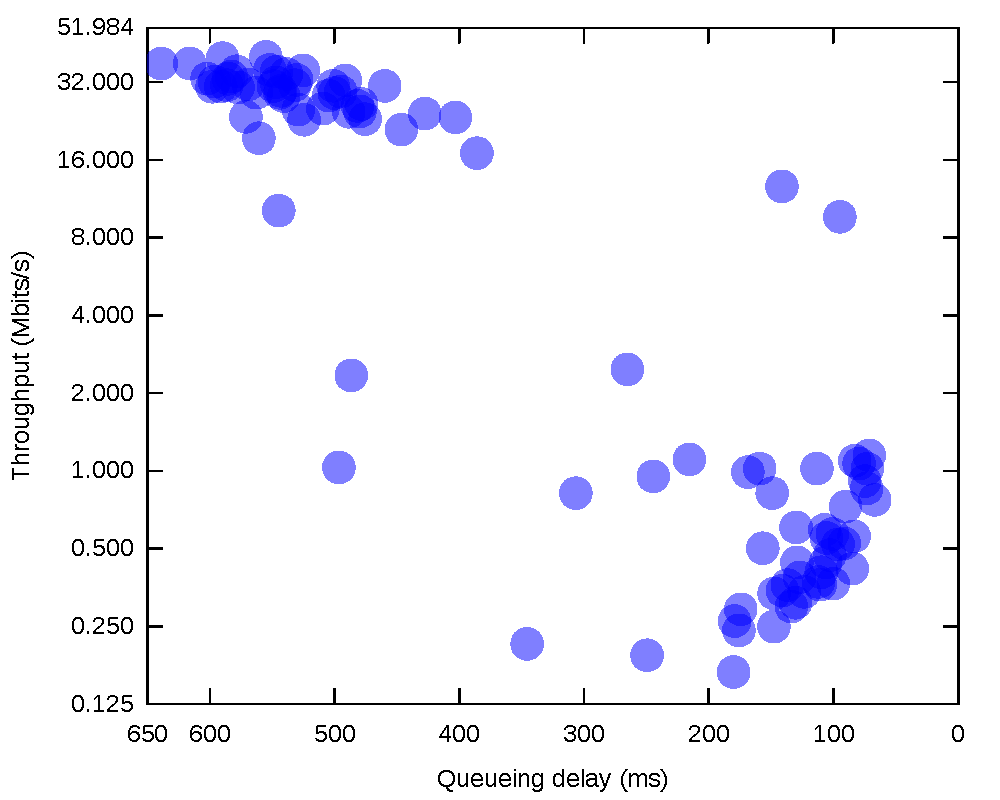
\includegraphics[width=3.3 in]{optimality-runs.pdf}}\only<3>{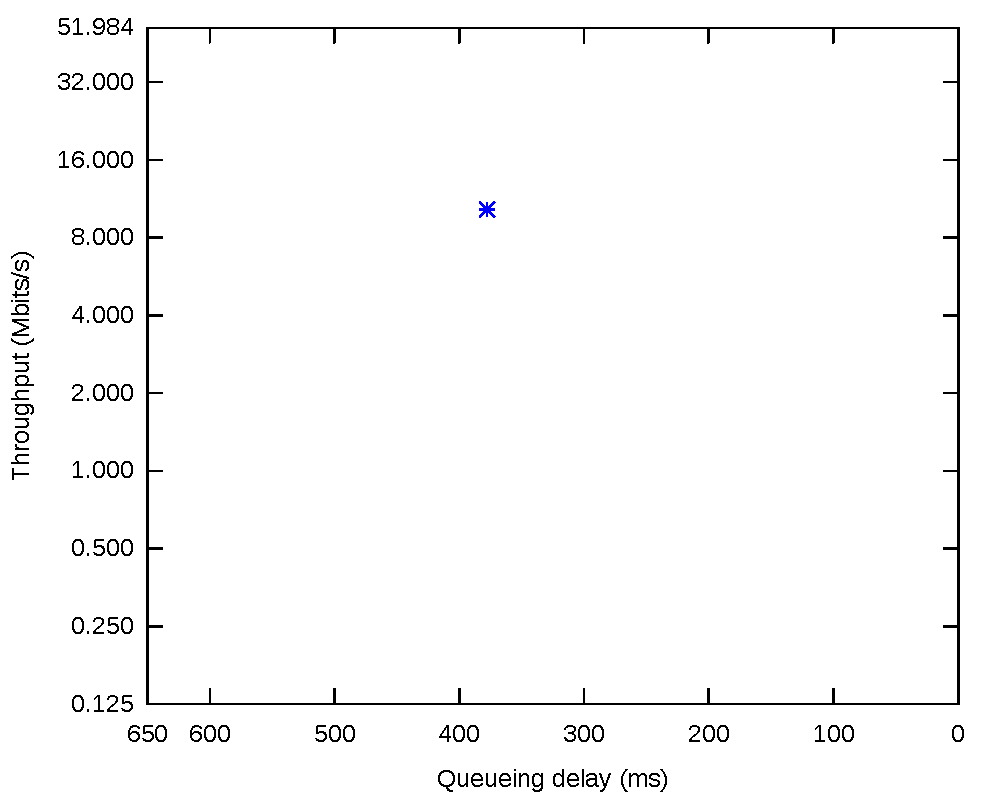
\includegraphics[width=3.3 in]{optimality-median.pdf}}\only<4>{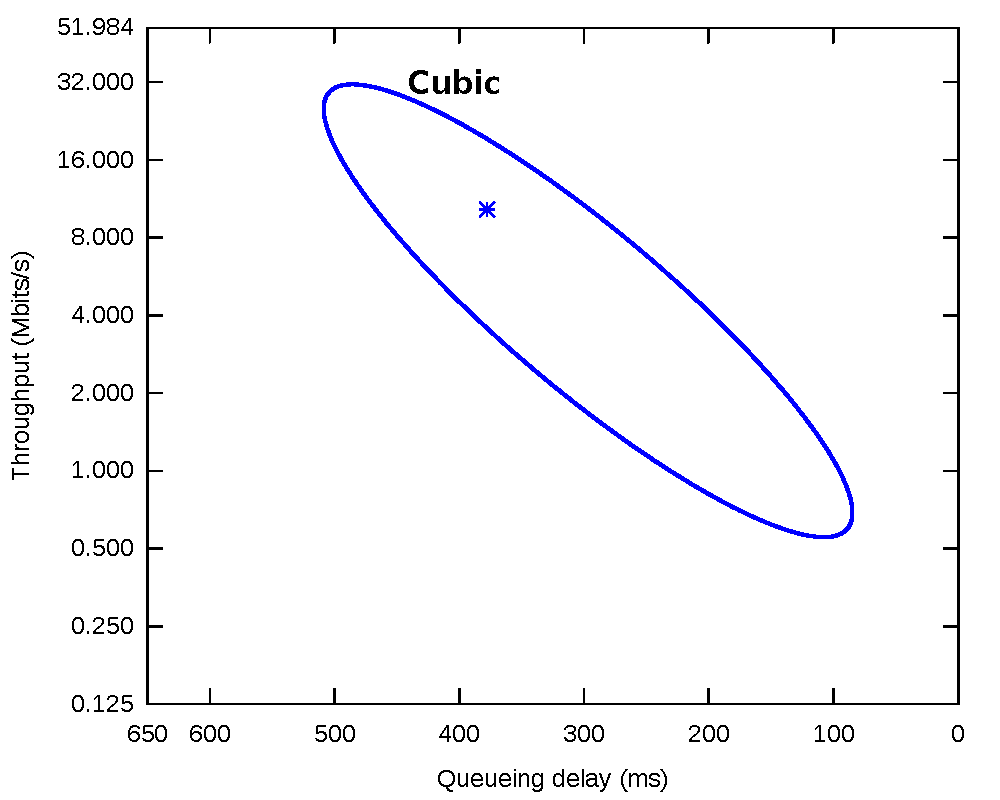
\includegraphics[width=3.3 in]{optimality-cubic.pdf}}\only<5>{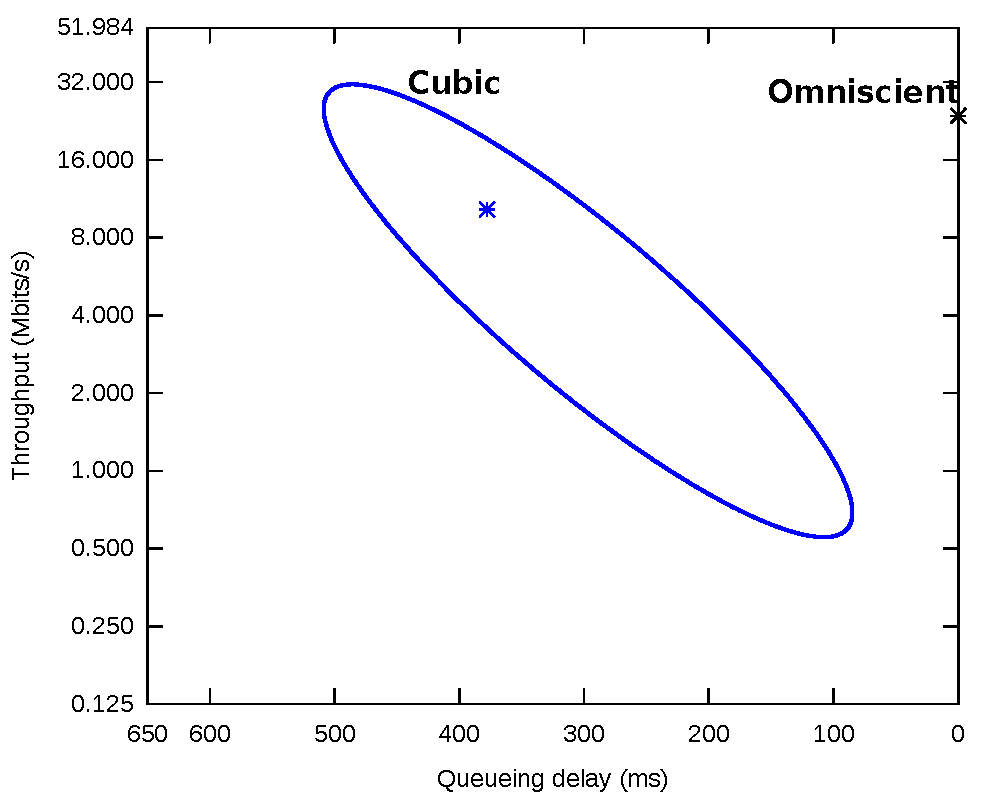
\includegraphics[width=3.3 in]{optimality-omni.pdf}}\only<6>{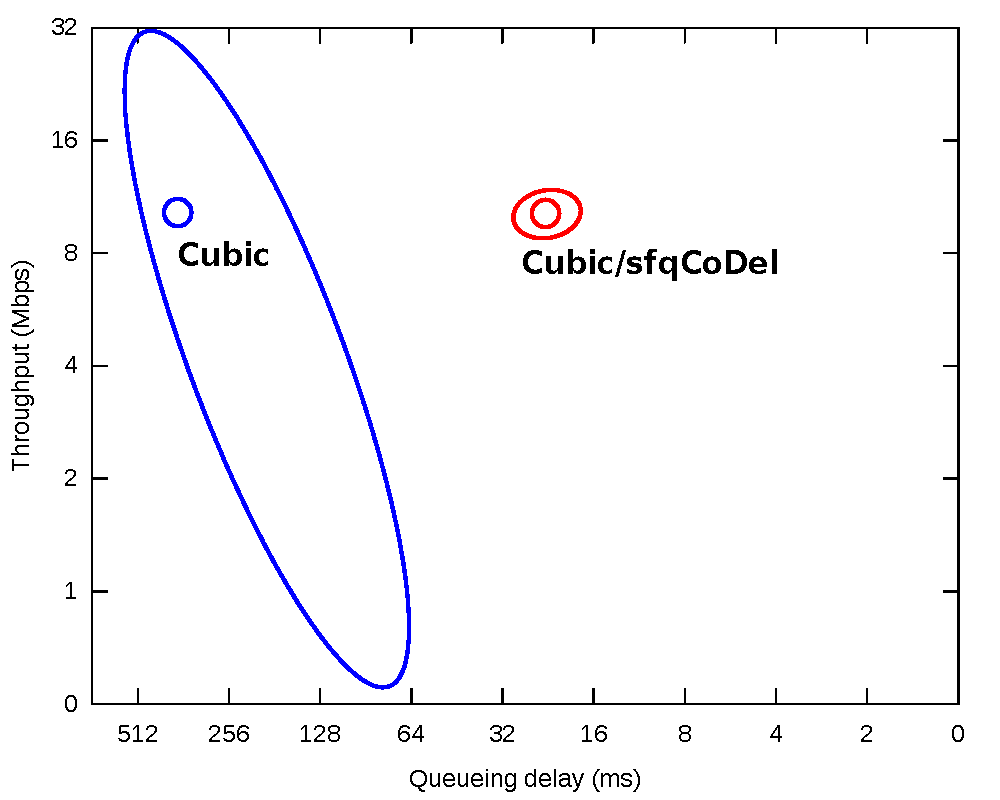
\includegraphics[width=3.3 in]{optimality-codel.pdf}}\only<7>{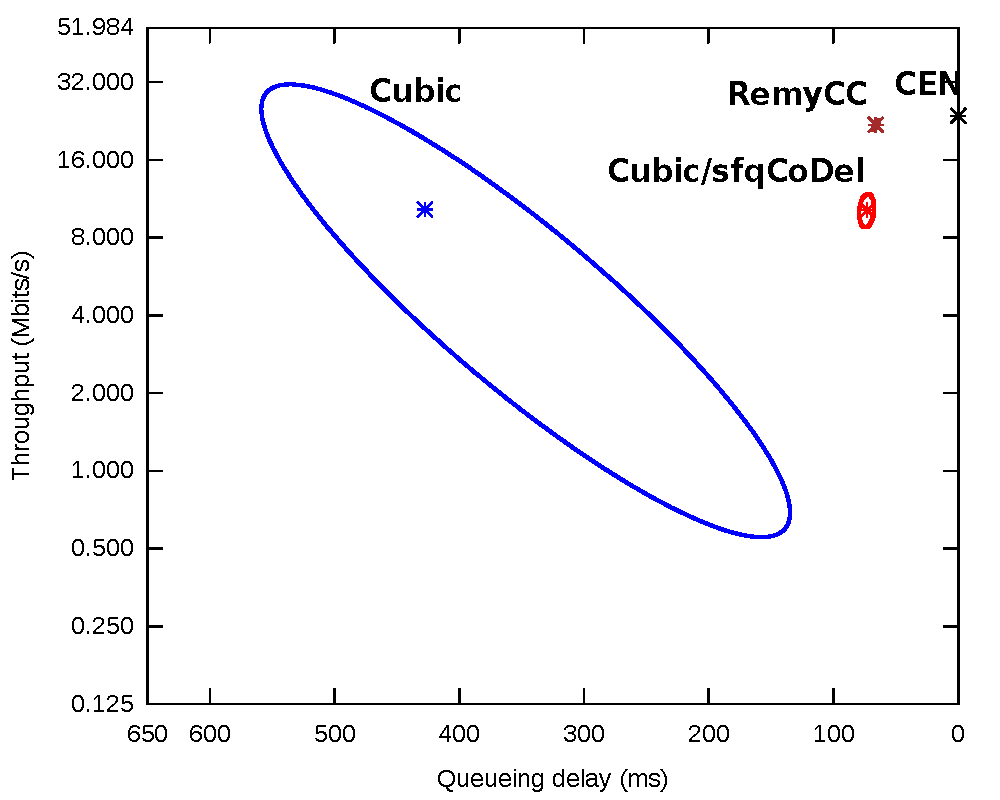
\includegraphics[width=3.3 in]{optimality-remy.pdf}}

\end{centering}
\end{frame}
